% This is samplepaper.tex, a sample chapter demonstrating the
% LLNCS macro package for Springer Computer Science proceedings;
% Version 2.20 of 2017/10/04
%
\documentclass[a4paper]{llncs}
%
\usepackage{graphicx}
% Used for displaying a sample figure. If possible, figure files should
% be included in EPS format.
%
% If you use the hyperref package, please uncomment the following line
% to display URLs in blue roman font according to Springer's eBook style:
% \renewcommand\UrlFont{\color{blue}\rmfamily}
\usepackage[english]{babel}
\usepackage[autostyle]{csquotes}
\usepackage[sorting=ynt,sortcites=true,backend=bibtex8,doi=false,maxnames=4,isbn=false,firstinits=true]{biblatex}
\addbibresource{reference}

\usepackage{hyperref}
\hypersetup
{
  bookmarks       = true,
  unicode         = true,
  pdftitle        = "Practical Type Blurring",
  pdfauthor       = "Ta Thanh Dinh", %auteur du document
%   pdfsubject      = "A Conceptual Approach for Message Format Extraction",
  pdftoolbar      = true, %barre d'outils non visible
  pdfmenubar      = true, %barre de menu visible
  pdfhighlight    = /O, %effet d'un clic sur un lien hypertexte
  colorlinks      = true, %couleurs sur les liens hypertextes
%   pdfpagemode = None, %aucun mode de page
%   pdfpagelayout = SinglePage, %ouverture en simple page
  pdffitwindow    = true, %pages ouvertes entierement dans toute la fenetre
  linkcolor       = red, %couleur des liens hypertextes internes
  citecolor       = green, %couleur des liens pour les citations
  urlcolor        = cyan, %couleur des liens pour les url
%   pagebackref=true
%   bookmarksdepth  = 3
}

\usepackage{listings}
\lstset{basicstyle=\small\ttfamily,showspaces=false,frame=tb}
\lstloadlanguages{C,C++,[x86masm]Assembler}

\usepackage{cleveref}

\begin{document}
%
\title{Practical Type Blurring}
%
%\titlerunning{Abbreviated paper title}
% If the paper title is too long for the running head, you can set
% an abbreviated paper title here
%
\author{Ta Thanh Dinh}
%
\authorrunning{Ta Thanh Dinh}
% First names are abbreviated in the running head.
% If there are more than two authors, 'et al.' is used.
%
\institute{
\email{tathanhdinh@gmail.com}}
%
\maketitle              % typeset the header of the contribution
%
\begin{abstract}
High-level type reconstruction is an important step in machine code decompilation.
Researchers show possibilities of mapping untyped machine-dependent
primitives into types of a C-like type system.


We show that the techniques used for type reconstruction can be bypassed,
and we claim that the bypass is always possible given \emph{semantics gap} between
type systems of high-level and machine language.
% \keywords{First keyword  \and Second keyword \and Another keyword.}
\end{abstract}
%
%
%
\section{Introduction}
Binary code type inference is to restore high-level type information of variables,
functions from machine codes. It is useful for reverse code engineering (e.g.
decompilation) or static binary rewriting/instrumentation, just to name a few.
Type reconstruction is available in several binary analysis
tools~\cite{noauthor_hex-rays_nodate, noauthor_jeb_nodate, noauthor_ghidra_nodate}
as a result of machine code decompilation. Academic research includes~\cite{mycroft_type-based_1999}
which was probably the pilot paper on the domain, an extension supporting
a limited form of subtyping is presented in~\cite{lee_tie_2011}, a survey of
research up until 2015 is given in~\cite{caballero_type_2016}. Recent
directions are using machine learning~\cite{maier_typeminer_2019} or statistical
language model~\cite{katz_estimating_2016}. All approaches tend to output a C-like type system.

Basically, the type inference starts by detecting high-level variables from
machine-dependent primitives: local variables are stored in function stack frame,
parameters are passed from registers, see~\cite{balakrishnan_wysinwyx_2007} for example.
Type constraints are generated then through the use of these variables. Finally,
the constraints are solved, each variable is annotated with a type given by the solver.

This bird view about binary code type reconstruction may give an impression that the
research domain has been well established already, the incorrectness comes from foreign
reasons: binary code disassembly, high-level variable detection, etc.
But there are more intrinsic problems, as we claim below.

\emph{First}, there is a common agreement that type information is removed through compilation~\cite{lee_tie_2011,caballero_type_2016,lin_automatic_2010},
but there is no explicit explication of why and how some type information is not needed
(so removed) in machine codes, actually not all type information can be restored.

\emph{Second}, while some researchers unify data structure reverse engineering with
type reconstruction~\cite{caballero_type_2016, caballero_polyglot_2007}, types do not
always attach with storage specific primitives (e.g. \texttt{int} is some \texttt{32-bit}
signed integer stored in a register or stack). The storage-based point of view though
mostly correct in low-level languages like C, does not reveal the nature of types. In
some languages other than C, types can be zero-sized~\cite{noauthor_phantom_nodate},
another example is \emph{regions}~\cite{grossman_region-based_2002} which have no
storage imprint.

The binary type reconstruction is influenced by \emph{Algorithm W} used originally to
type check/inference for programs of Hindley-Milner's type system (abbr. HM)~\cite{milner_theory_1978,hindley_principal_1969,cardelli_basic_1987}.
While the supposed target is a C-like type system, some authors claim to replicate
the result of \emph{principal types}~\cite{damas_principal_1982,hindley_principal_1969}
by recovering \emph{the most precise yet conservative} type~\cite{lee_tie_2011}.
Such a result is sound in a limited context only, C's type system is not HM: there
are functions that are trivially typed in C by casting, but not typeable in HM's.
Actually, it is not rare to observe type inconsistency in decompilation results
of security tools.

\paragraph{Contribution}
We first discuss the type information loss in compilation and some cases
where assigning a high-level \emph{type} for a low-level primitive
is not possible. Though this part is not novel, we bring it to the context
of binary code analysis to show limits of type reconstruction. Next, we present
a proof-of-concept C compiler which tries to hide types from reconstruction techniques described
in current researches.

\section{Type information loss}
Type system of a language can be considered as a set or rules about constraints
on programs of this language. On statically typed languages, the constraints
can be mechanically checked and proved without running the program, it helps
avoid bugs as Robin Milner's famous slogan~\textquote{well-type program cannot go wrong}~\cite{milner_theory_1978}.

There exists at least two sources information loss: \emph{type erasure} and
\emph{data indistinguishability}~\cite{noauthor_struct_nodate}, happening at
different phases of compilation.

\subsection{Type erasure}
Once the program is type checked, the type information is normally not needed for
evaluation (i.e. running program): the compiler can select a consistent machine-dependent
representation for each high-level type, this representation may only have little
relation with the original type but it does not violate the fact that the program
is checked (then safe).

\begin{example}\label{exa:typed_enum}
\texttt{C++}'s typed enum.

\begin{lstlisting}[frame=lines, language={C++}]
enum E { one = 1, two };
void foo(enum E e) {
  switch (e) {
  case E::one:
  case E::two:
    printf("ok\n");
    break;

  default: assert(false);
  }
}

enum E bar() {...return some enum E }

int main() {
  enum E e = bar(); foo(e);
  return 0:
}
\end{lstlisting}

The program is safe when type-checked: \texttt{assert(0)} will
never be reached when the program runs. In machine code, we may observe that
\texttt{foo} is a function accepting a \texttt{32-bit} signed integer, i.e. information about
\texttt{enum E} type is erased. However there is no need to add runtime
checking for the case where \texttt{foo} is passed an argument of value not in \texttt{enum E}
(e.g. \texttt{3}), this case is eliminated by the compiler's type checker.
\end{example}

\subsection{Data indistinguishability}
When generating binary code for a specific hardware/operating system, the compiler will
use a consistent representation for low-level primitives (e.g. registers used in
function parameters or return value, alignment for fields of aggregate types), so that
the output binary can be used by other programs on the same system. It it possible that
two types are distinguished at high-level but they have the same data representation
at low-level.

\begin{example}\label{exa:register_struct}
Small struct passing.

\begin{lstlisting}[frame=lines, language={C}]
struct S { int a; int b; };
int foo(struct S s) {
  return s.a + s.b;
}

int bar(long long l) {
  return (int)l + (int)(l >> 32);
}
\end{lstlisting}

Under System V AMD64 ABI~\cite{lu_system_nodate}, the aggregate type \texttt{S}
has class \texttt{INTEGER}: the argument \texttt{s} is passed just in register \texttt{rdi}.
At the ABI level, \texttt{foo} and \texttt{bar} is interchangeable, but they are not at
the type level.
\end{example}

\subsection{Untypeable}

There is no type casting in Hindley-Milner's type system (abbr. HM), so when using a variant of
\emph{Algorithm-W}~\cite{milner_theory_1978} for binary code type inference, the output (as a
C program without type casting) may not exist: there are programs which are
trivially typed in C, but not in HM.

\begin{example}\label{exa:untypeable}
Untypeable function.
\begin{lstlisting}[frame=topline, language={C}]
int foo(int i, int *f) {
  return ((int (*)(int (*)(int, int*), int))f)(foo, i);
}
\end{lstlisting}
Disassembled code:
\begin{lstlisting}[frame=bottomline, language={[x86masm]Assembler}]
0x0     55                               push rbp
0x1     48 89 e5                         mov rbp, rsp
0x4     48 83 ec 10                      sub rsp, 0x10
0x8     89 7d fc                         mov [rbp-0x4], edi
0xb     48 89 75 f0                      mov [rbp-0x10], rsi
0xf     48 8b 45 f0                      mov rax, [rbp-0x10]
0x13    8b 75 fc                         mov esi, [rbp-0x4]
0x16    48 bf 00 00 00 00 00 00 00 00    mov rdi, 0x0
0x20    ff d0                            call rax
0x22    48 83 c4 10                      add rsp, 0x10
0x26    5d                               pop rbp
0x27    c3                               ret
\end{lstlisting}

From disassembled code, it is direct to detect that the second argument
of \texttt{foo} is of functional type (since \texttt{call rax} at address \texttt{0x20}),
but assigning an functional type for \texttt{f} is not possible.
\end{example}

The inevitability of type information loss means that the binary code
type reconstruction cannot always reaches the notion of
\emph{the most precise yet conservative type}~\cite{lee_tie_2011}. Since
compilation is a \textquote{many-to-one mapping}~\cite{mycroft_type-based_1999},
real world decompilers simply look for one of possible maps,
sometimes they accept even inconsistencies in reconstructed types.

\section{Untyped C}



% \emph{well-type program cannot go wrong}, or even leads to better optimization.

\subsection{A Subsection Sample}
Please note that the first paragraph of a section or subsection is
not indented. The first paragraph that follows a table, figure,
equation etc. does not need an indent, either.

Subsequent paragraphs, however, are indented.

\subsubsection{Sample Heading (Third Level)} Only two levels of
headings should be numbered. Lower level headings remain unnumbered;
they are formatted as run-in headings.

\paragraph{Sample Heading (Fourth Level)}
The contribution should contain no more than four levels of
headings. Table~\ref{tab1} gives a summary of all heading levels.

\begin{table}
\caption{Table captions should be placed above the
tables.}\label{tab1}
\begin{tabular}{|l|l|l|}
\hline
Heading level &  Example & Font size and style\\
\hline
Title (centered) &  {\Large\bfseries Lecture Notes} & 14 point, bold\\
1st-level heading &  {\large\bfseries 1 Introduction} & 12 point, bold\\
2nd-level heading & {\bfseries 2.1 Printing Area} & 10 point, bold\\
3rd-level heading & {\bfseries Run-in Heading in Bold.} Text follows & 10 point, bold\\
4th-level heading & {\itshape Lowest Level Heading.} Text follows & 10 point, italic\\
\hline
\end{tabular}
\end{table}


\noindent Displayed equations are centered and set on a separate
line.
\begin{equation}
x + y = z
\end{equation}
Please try to avoid rasterized images for line-art diagrams and
schemas. Whenever possible, use vector graphics instead (see
Fig.~\ref{fig1}).

\begin{figure}
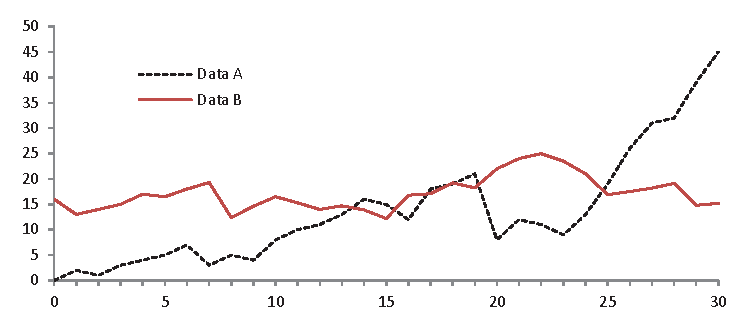
\includegraphics[width=\textwidth]{fig1.eps}
\caption{A figure caption is always placed below the illustration.
Please note that short captions are centered, while long ones are
justified by the macro package automatically.} \label{fig1}
\end{figure}

\begin{theorem}
This is a sample theorem. The run-in heading is set in bold, while
the following text appears in italics. Definitions, lemmas,
propositions, and corollaries are styled the same way.
\end{theorem}
%
% the environments 'definition', 'lemma', 'proposition', 'corollary',
% 'remark', and 'example' are defined in the LLNCS documentclass as well.
%
\begin{proof}
Proofs, examples, and remarks have the initial word in italics,
while the following text appears in normal font.
\end{proof}
For citations of references, we prefer the use of square brackets
and consecutive numbers. Citations using labels or the author/year
convention are also acceptable. The following bibliography provides
a sample reference list with entries for journal
articles~\cite{ref_article1}, an LNCS chapter~\cite{ref_lncs1}, a
book~\cite{ref_book1}, proceedings without editors~\cite{ref_proc1},
and a homepage~\cite{ref_url1}. Multiple citations are grouped
\cite{ref_article1,ref_lncs1,ref_book1},
\cite{ref_article1,ref_book1,ref_proc1,ref_url1}.
%
% ---- Bibliography ----
%
% BibTeX users should specify bibliography style 'splncs04'.
% References will then be sorted and formatted in the correct style.
%
% \bibliographystyle{splncs04}
% \bibliography{mybibliography}
%
% \begin{thebibliography}{8}
% \bibitem{ref_article1}
% Author, F.: Article title. Journal \textbf{2}(5), 99--110 (2016)

% \bibitem{ref_lncs1}
% Author, F., Author, S.: Title of a proceedings paper. In: Editor,
% F., Editor, S. (eds.) CONFERENCE 2016, LNCS, vol. 9999, pp. 1--13.
% Springer, Heidelberg (2016). \doi{10.10007/1234567890}

% \bibitem{ref_book1}
% Author, F., Author, S., Author, T.: Book title. 2nd edn. Publisher,
% Location (1999)

% \bibitem{ref_proc1}
% Author, A.-B.: Contribution title. In: 9th International Proceedings
% on Proceedings, pp. 1--2. Publisher, Location (2010)

% \bibitem{ref_url1}
% LNCS Homepage, \url{http://www.springer.com/lncs}. Last accessed 4
% Oct 2017
% \end{thebibliography}
\printbibliography
\end{document}
